\documentclass{article}
\usepackage[utf8]{inputenc}
\usepackage{graphicx}

\title{Sumas de Riemann}
\author{Brandonn Cruz\\Diego Barajas}
\date{September 2018}

\begin{document}

\maketitle

\section{Problema}
Calcular la integral de una función por medio del método de las Sumas de Riemann.\\
Para este ejercicio específico se trabaja sobre la Distribución Normal, por lo cual se calculará la integral a la función de densidad de probabilidad.

\section{Formalización}
\subsection{Entradas}
Dada la función $f(x) = \frac{1}{\sigma\sqrt[2]{2\pi}}e^{-\frac{(x-\mu)^2}{2 \sigma^2}}$, un valor z donde $0 > z > 3$ y un número r que dirá la cantidad de cifras decimales con que se quiere trabajar. Por ejemplo, si z tiene 2 cifras decimales, $r = 100$, pues $10^2 = 100$.
\subsection{Salidas}
Resultado de la integral $\int_{-3}^{z}\frac{1}{\sigma\sqrt[2]{2\pi}}e^{-\frac{(x-\mu)^2}{2 \sigma^2}}dx$.

\section{Implementación}
Para resolver la integral se usa el método de sumas de Riemann por lado izquierdo, derecho y centro. Es decir que se divide el eje x que está definido en el intervalo [-3,z], cada uno de los subintervalos se multiplicará por la función de densidad de probabilidad en un punto, dependiendo de si es el método por lado izquierdo, derecho o centro.\\
A continuación, se muestra un ejemplo en el que cada rectángulo corresponde a sumas por lado izquierdo, centro y derecho respectivamente.

\begin{figure}[h!]
\centering
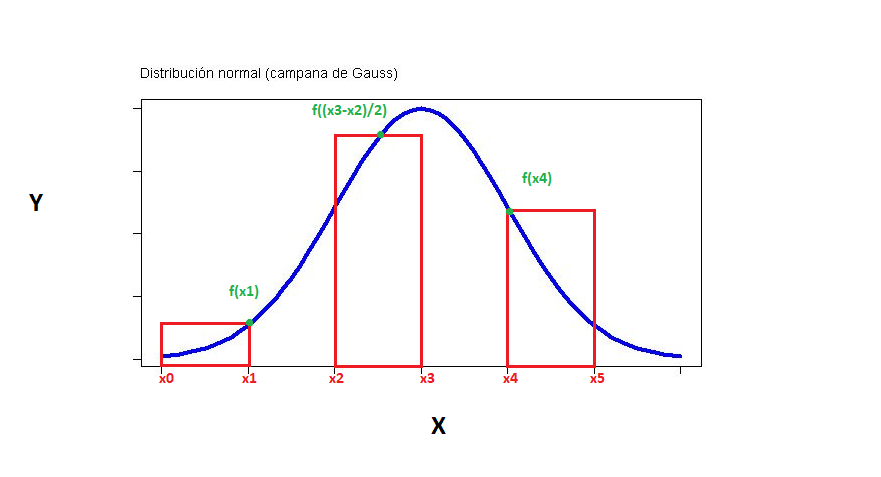
\includegraphics[scale=0.5]{sumas.png}
\caption{Sumas de Riemann por lado izquierdo, derecho y centro}
\label{fig:fisica}
\end{figure}
\newpage
El resultado de la integral por el lado izquierdo es:\\\\
$\sum_{i=1}^{n}{(xi-(xi-1))f(xi)}$\\\\
El resultado de la integral por centro es:\\\\
$\sum_{i=1}^{n}{(xi-(xi-1))f((xi-(xi-1))/2)}$\\\\
El resultado de la integral por el lado derecho es:\\\\
$\sum_{i=1}^{n}{(xi-(xi-1))f(xi-1)}$\\\\
Donde n es la cantidad de subintervalos en que se divide el intervalo [-3,z].

\section{Guía de compilación}
Ejecute el programa rimman.R. Las funciones son: derecha(z,r), izquierda(z,r) y centro(z,r).

\end{document}
